%!TEX root = ../thesis_phd.tex
%%%%%%%%%%%%%%%%%%%%%%%%%%%%%%%%%%%%%%%%%%%%%%%%%%%%%%%%%%%%%%%%%%%%%%%%%%%%%%%%
%neutrino_physics.tex: Chapter on neutrino physics:
%%%%%%%%%%%%%%%%%%%%%%%%%%%%%%%%%%%%%%%%%%%%%%%%%%%%%%%%%%%%%%%%%%%%%%%%%%%%%%%%
\chapter{Neural Networks}
\label{nnet_chapter}
%%%%%%%%%%%%%%%%%%%%%%%%%%%%%%%%%%%%%%%%%%%%%%%%%%%%%%%%%%%%%%%%%%%%%%%%%%%%%%%%

The field of machine learning is concerned with algorithms which can learn to make predictions from data.  Typically this involves some form of function approximation.  If the goal is to predict the output of a continuous function, the task is referred to as regression.  The task of separating examples into groups is called classification.

It is also common to separate machine learning approaches into two categories: supervised and unsupervised.  The supervised approach involves training an algorithm using a collection of examples for which the function output is known.  In unsupervised learning, algorithms can work to extract meaningful output from data where the function output is not known.

This thesis applies a supervised learning strategy for both classification of signal events and regression to approximate the energy of those events.

\section{Artificial Neural Networks}

An artificial neural network is a common tool used in classification and regression.  This class of algorithms draws inspiration from biological neurons.  Nervous systems of organisms are built up from a repeated structure of cells, called \textit{neurons}, which are connected to each other in order to transmit signals.  An example of a neuron can be seen in figure \ref{neuron}.  The base of a neuron is formed by a branching tree of \textit{dendrites} which receive signals from other neurons.  Signals are integrated and amplified in the cell body, then retransmitted through a long shaft, or \textit{axon}, to other neurons.  Intelligence is achieved by connecting many neurons which form a response to a given stimulus.

\begin{figure}[t]
  \begin{center}
    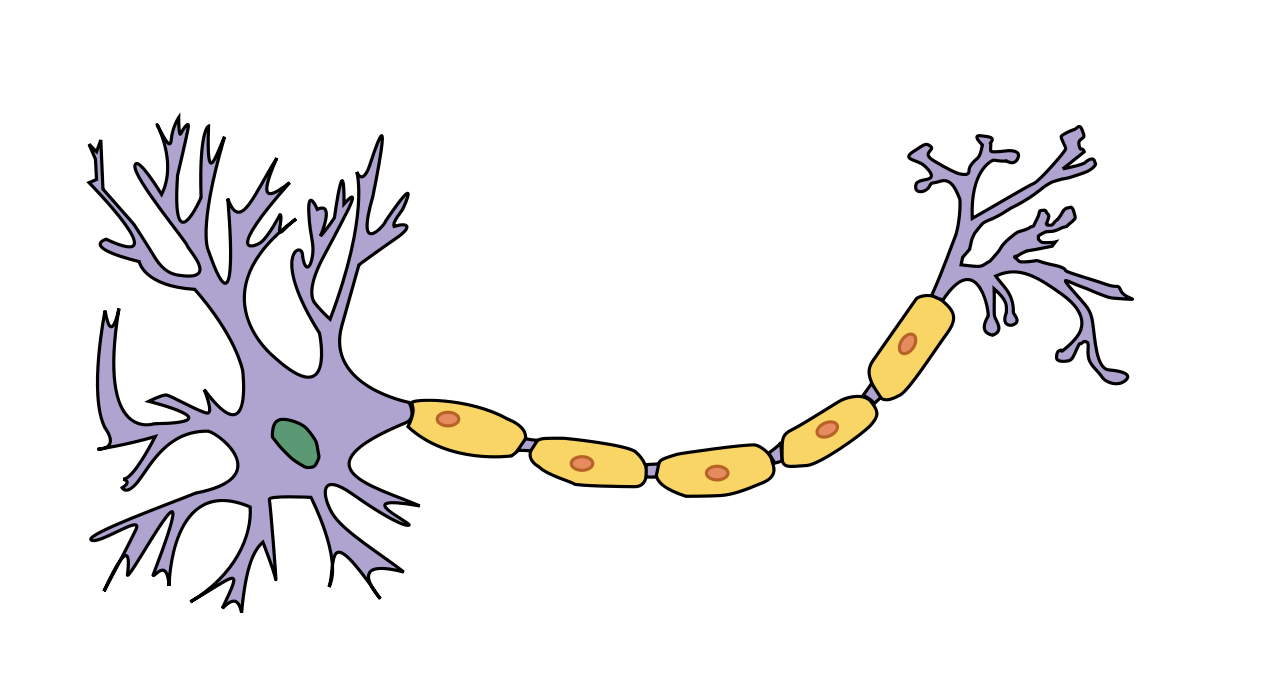
\includegraphics[width=\textwidth]{figures/figures/neuron.png}
  \end{center}
  \caption[A basic rendering of a biological neuron]{A basic rendering of a biological neuron.  Signals are received through the branching dendrites to the left of the image.  The cell body integrates and retransmits signals to other cells through the axon, which runs horizontally from left to right in the figure.  Biological nervous systems are based upon a repeated structure of neurons to carry signals over long distances.}

  \label{neuron}
\end{figure}


Artificial neural networks are designed to offer a crude approximation of a biological nervous system.  The basic unit of a neural network is called a \textit{node}.  Each is a function which computes an output value from a set of inputs.  Nodes are arranged into \textit{layers}, as seen in figure \ref{nnet}.  In graph theory terms, a neural network is a \textit{feedforward graph}, implying that information is passed forward to subsequent layers, but not backward.


In a \textit{fully connected} layer, all nodes in a given layer receive input from all nodes in the previous layer.  The response to each input is characterized by a set of weights; for node $i$ in layer $j$, the vector $w_{k}^{i,j}$ has an entry corresponding to each node $k$ in the previous layer.  Node response can thus be defined recursively:
\begin{equation}
z^{i,j} = \sum_{i=1}^{N_{(j-1)}} w_{k}^{i,j} z^{i,(j-1)}
\end{equation}

First layer? 

Feedforward graph. \cite{reed1999neural}

Each node is connected to nodes in the previous layers.

Node is represented by a vector of weights which determine response to input vector.


Output is result of nonlinearity

Layer structure, or architecture, is arbitrary.  Multilayer networks are popular.


Inputs can be anything.  Many cases involve input features which are engineered for a particular problem specification.  In the case of image processing, it is not uncommon to use all pixels from an image as the input layer.

\begin{figure}[t]
  \begin{center}
    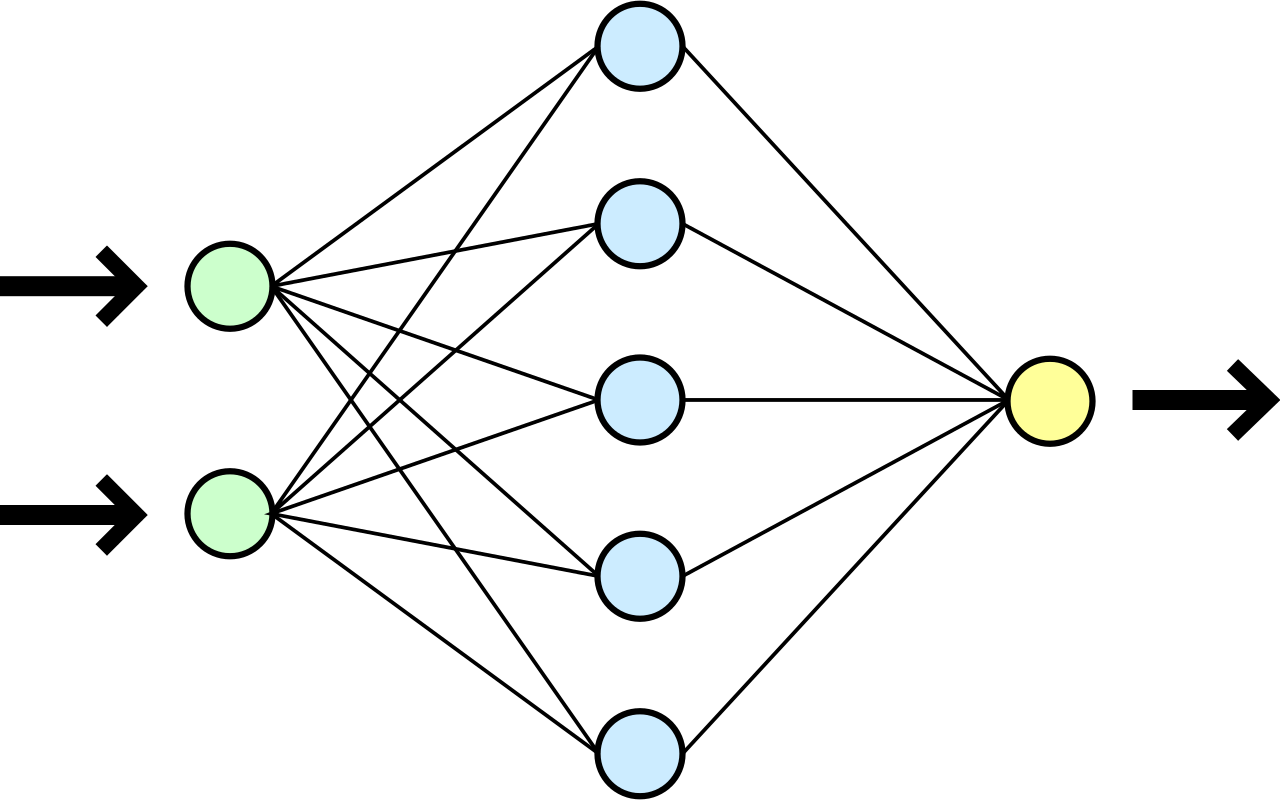
\includegraphics[width=0.6\textwidth]{figures/figures/basicNN.png}
  \end{center}
  \caption[Visualization of a simple neural network ]{Visualization of a simple neural network.  This network has an input layer (green) with two nodes, a hidden layer (blue) with five nodes, and an output layer (yellow) with one node.}

  \label{nnet}
\end{figure}


\section{Supervised Learning -- Backpropagation}


Minimize objective function

Gradient in each layer is propagated through to previous layer through chain rule.



\section{Neural Network Enhancements}

Convolution\cite{lecun1995comparison,lecun2010convolutional,krizhevsky2012imagenet} ... scan a filter... position independent... many filters of a particular size per layer... filters trained through backpropagation


\begin{figure}[t]
  \begin{center}
    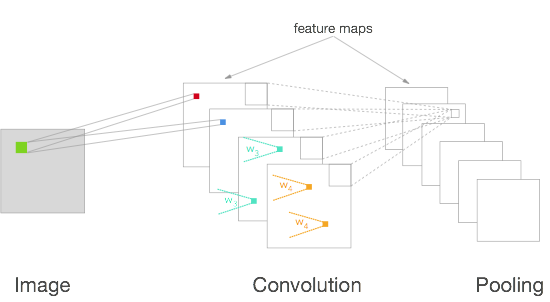
\includegraphics[width=0.6\textwidth]{figures/figures/convnet.png}
  \end{center}
  \caption[Example of a convolutional network ]{Example of a convolutional network.}

  \label{convnet}
\end{figure}



Pooling is used to reduce dimensionality. \cite{lecun2010convolutional} Image is downsampled by extracting a result from sub-regions of the image.  Two methods are commonly used, max pooling and average pooling.  Early results used non-overlapping pooling regions, although more recent efforts have seen good results from overlapping pooling regions \cite{krizhevsky2012imagenet}.




Network-in-network\cite{lin2013network} .... inception module \cite{szegedy2014going}

Dropout... regularization technique. \cite{hinton2014dropout}



%%%%%%%%%%%%%%%%%%%%%%%%%%%%%%%%%%%%%%%%%%%%%%%%%%%%%%%%%%%%%%%%%%%%%%%%%%%%%%%%
